% Options for packages loaded elsewhere
\PassOptionsToPackage{unicode}{hyperref}
\PassOptionsToPackage{hyphens}{url}
%
\documentclass[
  12pt,
]{article}
\usepackage{amsmath,amssymb}
\usepackage{iftex}
\ifPDFTeX
  \usepackage[T1]{fontenc}
  \usepackage[utf8]{inputenc}
  \usepackage{textcomp} % provide euro and other symbols
\else % if luatex or xetex
  \usepackage{unicode-math} % this also loads fontspec
  \defaultfontfeatures{Scale=MatchLowercase}
  \defaultfontfeatures[\rmfamily]{Ligatures=TeX,Scale=1}
\fi
\usepackage{lmodern}
\ifPDFTeX\else
  % xetex/luatex font selection
\fi
% Use upquote if available, for straight quotes in verbatim environments
\IfFileExists{upquote.sty}{\usepackage{upquote}}{}
\IfFileExists{microtype.sty}{% use microtype if available
  \usepackage[]{microtype}
  \UseMicrotypeSet[protrusion]{basicmath} % disable protrusion for tt fonts
}{}
\makeatletter
\@ifundefined{KOMAClassName}{% if non-KOMA class
  \IfFileExists{parskip.sty}{%
    \usepackage{parskip}
  }{% else
    \setlength{\parindent}{0pt}
    \setlength{\parskip}{6pt plus 2pt minus 1pt}}
}{% if KOMA class
  \KOMAoptions{parskip=half}}
\makeatother
\usepackage{xcolor}
\usepackage[margin=1in]{geometry}
\usepackage{graphicx}
\makeatletter
\def\maxwidth{\ifdim\Gin@nat@width>\linewidth\linewidth\else\Gin@nat@width\fi}
\def\maxheight{\ifdim\Gin@nat@height>\textheight\textheight\else\Gin@nat@height\fi}
\makeatother
% Scale images if necessary, so that they will not overflow the page
% margins by default, and it is still possible to overwrite the defaults
% using explicit options in \includegraphics[width, height, ...]{}
\setkeys{Gin}{width=\maxwidth,height=\maxheight,keepaspectratio}
% Set default figure placement to htbp
\makeatletter
\def\fps@figure{htbp}
\makeatother
\setlength{\emergencystretch}{3em} % prevent overfull lines
\providecommand{\tightlist}{%
  \setlength{\itemsep}{0pt}\setlength{\parskip}{0pt}}
\setcounter{secnumdepth}{5}
\usepackage{setspace} \usepackage{amsmath} \usepackage{graphicx} \usepackage{array} \usepackage{caption} \usepackage{longtable} \usepackage{booktabs} \usepackage{enumitem} \renewcommand{\arraystretch}{1} \captionsetup[table]{skip=5pt} \setstretch{1.5}
\ifLuaTeX
  \usepackage{selnolig}  % disable illegal ligatures
\fi
\usepackage[]{natbib}
\bibliographystyle{apalike}
\IfFileExists{bookmark.sty}{\usepackage{bookmark}}{\usepackage{hyperref}}
\IfFileExists{xurl.sty}{\usepackage{xurl}}{} % add URL line breaks if available
\urlstyle{same}
\hypersetup{
  pdftitle={Progress Report for Annual Review 22/23 - v2},
  pdfauthor={Zijian Zark Wang},
  hidelinks,
  pdfcreator={LaTeX via pandoc}}

\title{Progress Report for Annual Review 22/23 - v2}
\author{Zijian Zark Wang}
\date{August 08, 2023}

\begin{document}
\maketitle

\hypertarget{introduction}{%
\section{Introduction}\label{introduction}}

In this document, I present three pieces of work.

The first is a novel model of intertemporal choice. The model
incorporates attentional mechanism into the expected discounted utility
framework. It assumes that people have limited attention to allocate
across sequential outcomes and tend to pay more attention to the
outcomes with larger rewards. I show that it can explain a broad set of
decision anomalies, and present an axiomatic characterization.

The second is an experimental test on whether (and how) attentional
mechanism can influence intertemporal choice.

The third is an experiment aiming to test how people jointly evaluate
risky outcomes and efforts. The findings from this experiment can inform
the research in rational inattention. I am working on the experimental
program.

\hypertarget{attentional-discounted-utility}{%
\section{Attentional Discounted
Utility}\label{attentional-discounted-utility}}

\hypertarget{the-model}{%
\subsection{The Model}\label{the-model}}

Expected discounted utility framework has been widely used in behavioral
and economic research. Given a sequence of rewards
\(X_T=[x_0,x_1,...,x_T]\), which yields reward \(x_t\) in time period
\(t\),\footnote{I use uppercase letters to represent a sequence and
  lowercase letters to represent each element within the sequence.}
\(t \in \{0,1,...,T\}\), the expected discounted utility of \(X_T\) can
be calculated by\[
EDU(X_T)= \mathbb{E}\left[\sum_{t=0}^T d_t u(x_t)\right]
\]where \(d_t\) is the discounting factor of time period \(t\), reward
level \(x_t\) is a random variable defined on \(\mathbb{R}_{\geq 0}\),
\(u(.)\) denotes the decision maker's instantaneous utility function,
\(u'>0\), \(u''<0\). The time length of this sequence, denoted by \(T\),
is finite.

The aim of this section is to incorporate attentional mechanism into
this valuation process of reward sequences. I assume that a decision
maker allocates attention across sequential outcomes when processing
information about rewards, and attends more to the outcomes with larger
rewards. I define the models that contain such features as
\emph{Attentional Discounted Utility} (ADU). Previous studies exploring
the ADU setting include \citet{gershman_rationally_2020} and
\citet{noor_optimal_2022}. Specifically, I focus on a particular form of
ADU, which I term as \emph{ADU with Shannon cost function} (ADUS). ADUS
retains the architecture of expected discounted utility, but simply
modifies the conventional discounting factor \(d_t\) to \(w_t\), which I
refer to as attention weight hereafter, where

\begin{equation}\tag{1}\label{eq:wt}
w_t = \frac{d_t e^{u(x_t)/\lambda}}{\sum_{\tau=0}^T d_\tau e^{u(x_\tau)/\lambda}}
\end{equation}

In Equation (\ref{eq:wt}), \(w_t\) adopts a form resembling logistic
function. It indicates three properties of attention. First, the sum of
all \(w_t\) equals 1, indicating the attention that is available to be
allocated across sequential outcomes is limited. Second, \(w_t\) is
increasing in \(x_t\), indicating the decision maker is inclined to
allocate more attention to periods with larger potential rewards. This
is in line with existing evidence, suggesting people often pay much
attention to pleasant information and avoid to know unpleasant
information (e.g.~ostrich effect). Third, it appears that \(w_t\) is
anchored in \(d_t\). This indicates that the conventional discounting
factor \(d_t\) can represent the initial attention weight assigned to
each period, and the psychological process of attention adjustment
(converting \(d_t\) to \(w_t\)) is costly. The parameter \(\lambda\)
quantifies the cost of attention adjustment. Notably, \(w_t\) is
positive for every period \(t\) within the sequence.

I provide two rationales for Equation (\ref{eq:wt}). The first is based
on rational inattention theories. The second is an axiomatic theory. I
present the first here and discuss the second in Subsection \ref{axiom}.

The necessary notations and definitions are described as follows. Let
\(S_T=[s_0,s_1,...,s_T]\) be a potential realization of \(X_T\), and
\(\mathcal{S}(X_T)\) be the support of \(X_T\), i.e.~the smallest set
containing any potentially realized sequence \(S_T\), where
\(\mathcal{S}(X_T)\subseteq \mathbb{R}_{\geq 0}^{T+1}\). In each
\(S_T\), the attention weight assigned to period \(t\) is decided by a
weight function \(w(s_t)\). I follow Noor and Takeoka
\citetext{\citeyear{noor_optimal_2022}; \citeyear{noor_constrained_2023}}
to define the process that generates \(w(s_t)\) as \emph{constrained
optimal discounting}. The key assumption of constrained optimal
discounting process is that, when evaluating a reward sequence, the
decision maker wants to find an allocation policy for attention weights,
in order to maximize the anticipatory utility that she can obtain from
the sequence. Nonetheless, this attention re-allocation process triggers
a cognitive cost. She needs to balance the benefit of focusing on
periods containing larger rewards and the cognitive cost of shifting
attention. The formal definition is given by Definition 1.

\textbf{Definition 1}: Let \(W\) be the support of all possible weight
functions. Given a stochastic reward sequence \(X_T\), the following
optimization problem is called the \emph{constrained optimal
discounting} problem for \(X_T\):\[ 
\begin{aligned}
\max_{w\in W}  \quad & \sum_{S_T\in \mathcal{S}(X_T)}\sum_{t=0}^T w(s_t)u(s_t) - C(w) \\
s.t. \quad &  \sum_{S_T\in \mathcal{S}}\sum_{t=0}^T w(s_t)=m \\
& w(s_t)> 0, \forall t\in\{0,1,…,T\} \\
\end{aligned}
\]where \(m\) is a constant,
\(C:[0,m]^{T+1}\rightarrow \mathbb{R}_{>0}\) is called \emph{information
cost} function, \(\partial C/\partial w(s_t)>0\) and
\(\partial^2 C/\partial w(s_t)^2>0\). That is, the information cost is
increasing and convex in \(w(s_t)\).

In Definition 1, the cognitive cost of shifting attention is decided by
an information cost function \(C(.)\) . This implies that the cognitive
cost is generated by focusing on certain reward information. A
well-known specification of \(C(.)\) is the Shannon cost function,
proposed by \citet{matejka_rational_2015}. The Shannon cost function was
originally used to justify the multinominal logit model in discrete
choice analysis, and so far has been topical in rational inattention
literature. To construct this style of information cost function,
\citet{matejka_rational_2015} introduce three assumptions. The first is
that the sum of all weights is 1, i.e.~\(m\equiv1\). The second is,
before acquiring any information, the decision maker establishes an
initial weight allocation for different attributes (outcomes), which
remains invariant across states. The weights are then updated in a
manner consistent with Bayes rule. In ADU setting, it means
\(d_t=\sum_{S_T\in \mathcal{S}(X_T)} w(s_t)\). The third assumption is,
the information cost is linear to the information gains, measured by
Shannon mutual information. That
is,\[ C(w)= \lambda \sum_{S_T\in \mathcal{S}(X_T)}\sum_{t=0}^T w(s_t) \log\left(\frac{w(s_t)}{d_t p(S_T)}\right) \]where
\(\lambda\) is a parameter denoting unit cost of information
(\(\lambda>0\)), \(p(S_T)\) is the probability that \(S_T\) occurs. With
Shannon cost function, the constrained optimal discounting problem can
be easily solved by Lagrangian method, and the solution is the same as
Equation (\ref{eq:wt}). \footnote{In each certain state \(S_T\), \(w_t\)
  in Equation (\ref{eq:wt}) can be defined by
  \(w_t\equiv w(s_t)/p(S_T)\).}

\hypertarget{implications-in-intertemporal-choice}{%
\subsection{Implications in Intertemporal
Choice}\label{implications-in-intertemporal-choice}}

\hypertarget{adu-is-generally-consistent-with-hidden-zero-effect}{%
\subsubsection{ADU is generally consistent with ``hidden zero
effect''}\label{adu-is-generally-consistent-with-hidden-zero-effect}}

Suppose a decision maker faces a choice between a small sooner reward
(SS) and a larger later reward (LL). The hidden zero effect
\citep{magen_hidden-zero_2008} implies she should exhibit more patience
if both SS and LL are framed as sequences rather than being framed as
single-period rewards. For instance, consider SS\textsubscript{0}:
``receive £100 today'', and LL\textsubscript{0}: ``receive £120 in 6
months''. Suppose we also have

\setlength{\leftskip}{1cm}

SS\textsubscript{1}: ``receive £100 today and £0 in 6 months''

LL\textsubscript{1}: ``receive £0 today and £120 in 6 months''

\setlength{\leftskip}{0pt}

The hidden zero effect suggests people may be more likely to prefer
LL\textsubscript{1} over SS\textsubscript{1} than preferring
LL\textsubscript{0} over SS\textsubscript{0}. Subsequent research (e.g.
\citet{read_value_2017}) suggests the effect is asymmetric. That is,
shifting SS\textsubscript{0} to SS\textsubscript{1} and keeping
LL\textsubscript{0} unchanged do increase patience, whereas shifting
LL\textsubscript{0} to LL\textsubscript{1} and keeping
SS\textsubscript{0} unchanged cannot increase patience. This is
naturally compatible with attentional discounted utility.

To illustrate, imagine that the framing of sequence length can influence
how the decision maker may perceive it. For SS\textsubscript{0}, the
decision maker perceives the length of sequence as ``today''; for
SS\textsubscript{1}, she perceives the length as ``6 months''. In the
former case, she can allocate no attention to the future; while in the
latter case, she needs to pay some attention to future periods, which
contain no reward. Thus, the attention allocated to the current period
decreases when shifting from SS\textsubscript{0} to SS\textsubscript{1}
(given total amount of attention is limited). This leads to a decrease
in the value of sequence. By contrast, shifting from LL\textsubscript{0}
to LL\textsubscript{1} does not change the length of sequence, thus does
not change the value.

One might wonder for a period with no reward, why the attention weight
may still be positive (``why should I pay attention to a period when
there is no reward present''). The hidden zero effect provides an
empirical reason. Additionally, from the theoretical view, attention
acts as a filter that determines which information could enter awareness
or working memory.\footnote{Such a view can be traced back to the
  bottleneck theories of attention, which starts from
  \citet{broadbent_perception_1958}.} If the decision maker is aware
about the information that the reward for a certain period is zero, it
implies attention may have already been directed to that period.

Hereafter, I focus on ADU with Shannon cost function (ADUS) and document
five implications of the ADUS model in intertemporal choice. Each of
them can be precisely proved.

\hypertarget{the-requirement-of-magnitude-effect-on-utility-function-can-be-relaxed-under-adus}{%
\subsubsection{The requirement of magnitude effect on utility function
can be relaxed under
ADUS}\label{the-requirement-of-magnitude-effect-on-utility-function-can-be-relaxed-under-adus}}

In conventional discounted utility models, to make the magnitude effect
holds true, the elasticity of utility function needs to be increasing
with reward level \citep{loewenstein_anomalies_1992}. This requirement
might be too strong so that many commonly used utility functions (such
as power and CARA utility functions) does not satisfy it. By contrast,
note in Equation (\ref{eq:wt}), \(w_t\) is increasing in \(x_t\). This
implies that when comparing SS and LL, the decision maker could exhibit
more patience toward larger reward levels, which relaxes the requirement
for the magnitude effect \citep{noor_intertemporal_2011}.

To illustrate how specifically ADUS relaxes this requirement, we should
derive how a delayed reward is valued in ADUS. Suppose the value of
``receive a certain reward \(x_T\) in period \(T\)'' is calculated by
\(w_T \cdot u(x_T)\). Then assuming the initial attention weight is in
exponential style, that is \(d_t\equiv\delta^t\) (\(0<\delta\leq1\)), we
should have

\begin{equation}\tag{2}\label{eq:w2}  
w_T = \frac{1}{1+G(T)e^{-u(x_T)/\lambda}}  
\end{equation}

and

\begin{equation}\tag{3}\label{eq:gt} 
G(T) = \left\{ 
\begin{aligned} 
& \frac{1}{1-\delta}(\delta^{-T}-1) \; ,& 0<\delta<1\\ 
& T\; ,& \delta=1
\end{aligned} \right. 
\end{equation}

It can be proved that, if Equation (\ref{eq:w2}) and (\ref{eq:gt}) are
both satisfied, for all \(x_T>0\), power utility function
\(u(x_T)={x_T}^\gamma\) with \(0<\gamma<1\), satisfies the curvature
requirement for magnitude effect, and when \(x_T\) is greater than a
positive finite number, CRRA utility function
\(u(x_T)=1-e^{-\gamma x_T}\) with \(\gamma>0\), also satisfies it.

\hypertarget{adus-specifies-a-novel-condition-for-common-difference-effect}{%
\subsubsection{ADUS specifies a novel condition for common difference
effect}\label{adus-specifies-a-novel-condition-for-common-difference-effect}}

According to the common difference effect
\citep{loewenstein_anomalies_1992}, suppose a decision maker is
indifferent between SS and LL, increasing the time delay before
receiving the reward in both options by a same amount can lead the
decision maker to prefer LL over SS.

The ADU models provide an alternative account for common difference
effect. Given attention is limited, when the delay of reward is
extended, that is, we insert some periods with zero reward into the
existing sequence, these newly inserted periods will grab attention from
other periods. As people tend to attend more to periods with larger
rewards, the period when the reward is delivered in LL will experience
less attention being diverted compared to that in SS. This disparity in
attention weighing can lead to a preference for LL over SS.

Regarding Shannon cost function, assuming initial time preference is
stationary, i.e.~\(d_t=\delta^t\), we can derive from Equation
(\ref{eq:w2}) and (\ref{eq:gt}) the conditions for common difference
effect. Clearly, if \(\delta=1\), the attention weight \(w_T\) will
follow a hyperbolic style. In this case, the common difference effect
will always hold true.

If \(0<\delta<1\), the ADUS specifies a novel condition for common
difference effect. To illustrate, suppose SS is ``receive a certain
reward \(x_s\) in period \(t_s\)'' and LL is ``receive a certain reward
\(x_l\) in period \(t_l\)'', where \(x_l>x_s>0\), \(t_l>t_s>0\). To make
the common difference effect hold true, we need
\(v(x_l)-v(x_s)+\ln\frac{v(x_l)}{v(x_s)}>-(t_l-t_s)\ln\delta\). That is,
when the decision maker is impatient, she performs the common difference
effect if and only if \emph{the difference between SS and LL in reward
level is significantly larger than that in time delay}.

\hypertarget{discount-function-may-be-concave-for-the-near-future-and-convex-for-the-far-future}{%
\subsubsection{Discount function may be concave for the near future and
convex for the far
future}\label{discount-function-may-be-concave-for-the-near-future-and-convex-for-the-far-future}}

Most models of time discounting (e.g.~hyperbolic and quasi-hyperbolic
discounting) assume a convex discount function. However, some studies
suggest the discount function may be concave for the near future and
convex for the far future
\citep{onay_intertemporal_2007, takeuchi_non-parametric_2011, dejarnette_time_2020}.
This property can emerge in ADUS due to the attention weight following a
logistic-like function.

In Equation (\ref{eq:w2}), \(w_T\) produces this style of discount
function when \(x_T\) is greater than a positive finite number. This is
illustrated in Figure \ref{fig:plot-discount-value}(a).

\begin{figure}
  \centering
  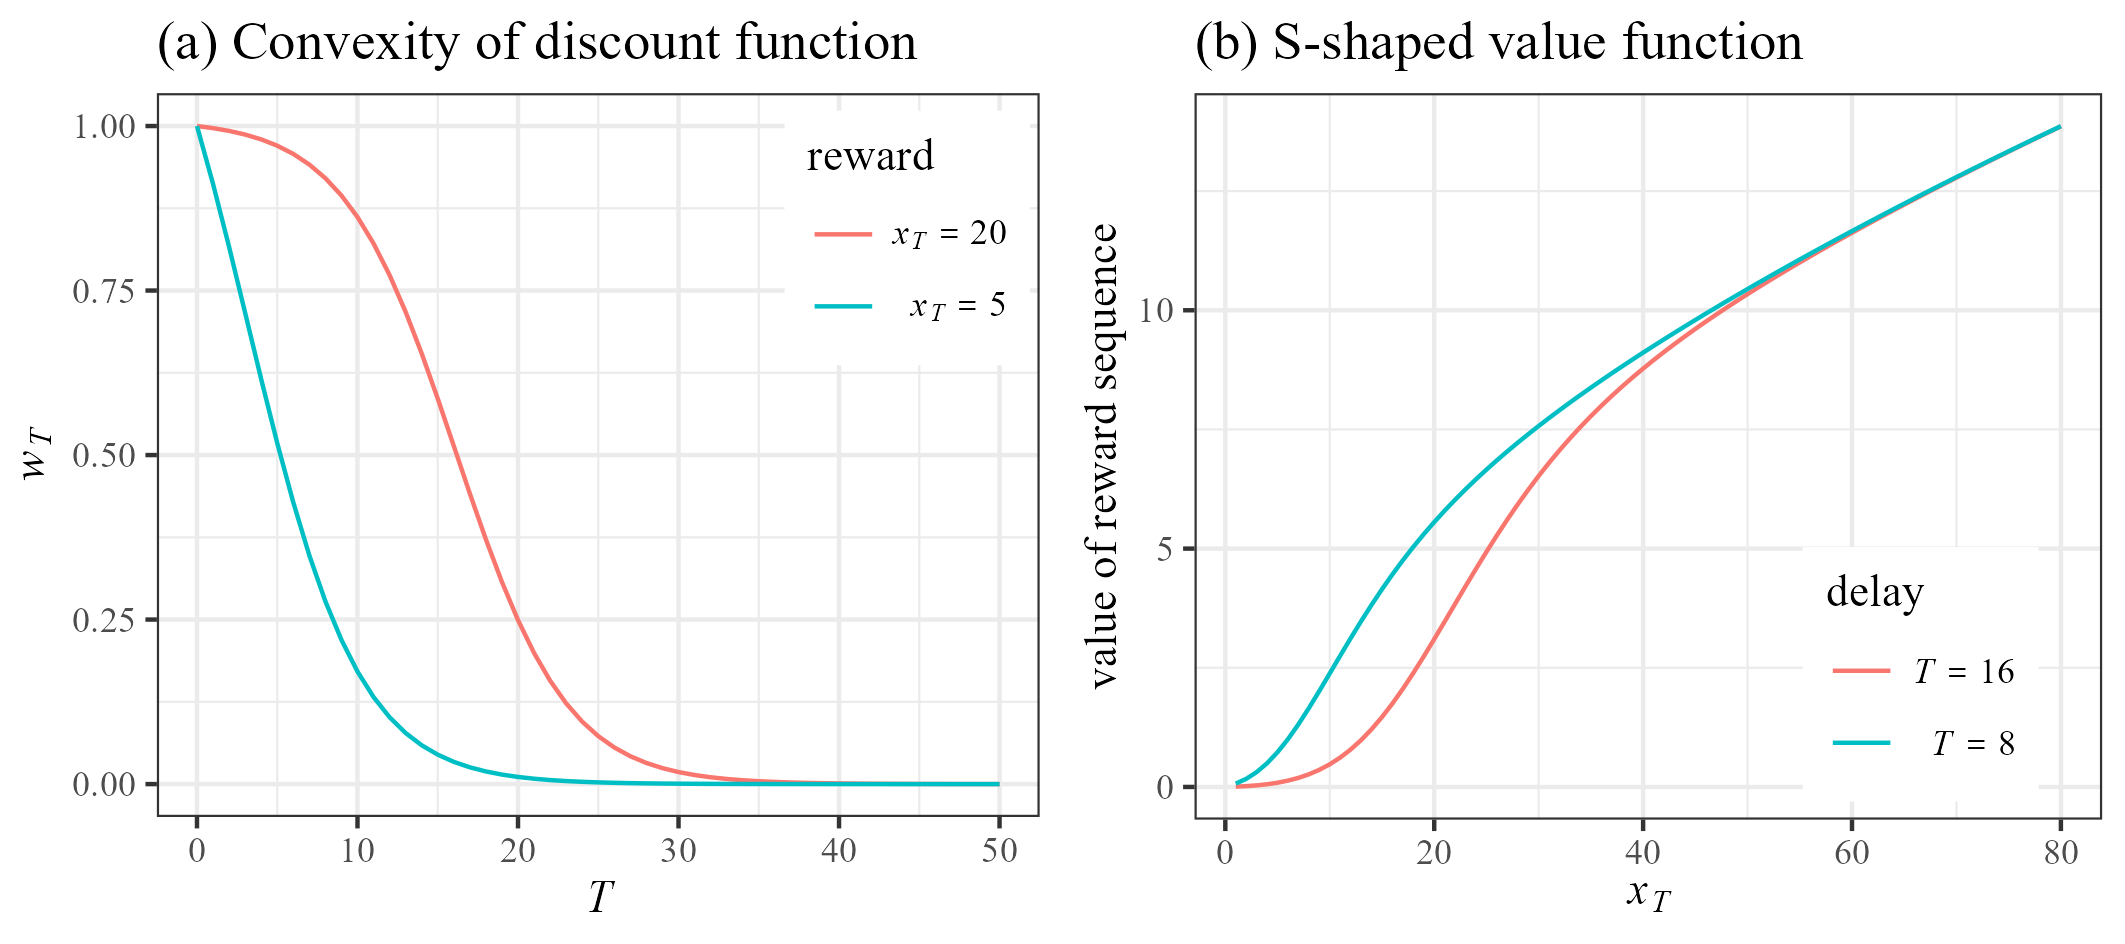
\includegraphics{images/plot-discount-value.png}
  \caption{Simulation results for choices between SS and LL. Value of reward sequence is calculated by $w_T\cdot u(x_T)$, where $w_T$ is calculated using Equation (2), $\delta=0.75$, $\lambda=1$, utility funtion $u(x)=x^{0.6}$.}
  \label{fig:plot-discount-value}
\end{figure}

\hypertarget{adus-offers-an-alternative-account-for-s-shaped-value-function}{%
\subsubsection{ADUS offers an alternative account for S-shaped value
function}\label{adus-offers-an-alternative-account-for-s-shaped-value-function}}

The S-shaped value function has been widely adopted by behavioral
economists. Some theories justifies it by reference-dependent utility
\citep{kahneman_prospect_1979, koszegi_model_2006}, while some others by
efficient coding of numerical values \citep{frydman_efficient_2021}. I
offer an account based on selective attention to sequential outcomes.

Imagine that a decision maker faces a choice between two lotteries. At
the moment when the choice is made, she does not receive any money from
either option. Thus, she may perceive the outcome of each option as
something that will happen in the future. She allocates attention
between the current period, which offers no reward, and the future
period when she could receive the money. When the amount of money that
she could receive is increased, not just does its utility increases, but
her attention is more directed towards that particular period.

Assuming the decision maker perceives the outcome will be realized in
period \(T\), and in a certain state, the option she chooses yields
reward \(x_T\). We can use Equation (\ref{eq:w2}) to derive the value
function, i.e.~\(w_T\cdot u(x_T)\). Both utility function \(u(.)\) and
attention weight \(w_T\) exhibit diminishing sensitivity to the reward
outcome \(x_T\). However, when the reward is small enough, their product
may be convex . Notably, when the curvature of utility function
satisfies a certain condition, or the unit cost of information
\(\lambda\) is small enough, we can obverse a S-shaped value function.
Figure \ref{fig:plot-discount-value}(b) illustrates this.

\hypertarget{inattentive-decision-makers-perform-less-inconsistent-behaviors}{%
\subsubsection{Inattentive decision makers perform less inconsistent
behaviors}\label{inattentive-decision-makers-perform-less-inconsistent-behaviors}}

Imagine that a decision maker faces a task of allocating consumption
budget \(B\) across multiple periods, and in each period, she makes a
new consumption plan to optimize her overall attentional discounted
utility. Suppose she starts in period 0, then the task can be formulated
as the following optimization problem:

\[
\max_{c_0,...,c_T}\;\sum_{t=0}^T w_t\cdot u(c_t) \qquad s.t.\;\sum_{t=0}^T c_t=B  
\]

where \(c_t\) is consumption in period \(t\), \(w_t\) is the attention
weight, which is calculated with ADUS. I develop a numerical method to
solve this optimization problem.

Previously, researchers often employ ``present bias''
\citep{laibson_golden_1997} or ``naiveté'' \citep{odonoghue_doing_1999}
to account for the phenomenon of dynamic inconsistency in this context.
I provide an account based on attention weight updating.

I categorize each decision maker into two types based on how they
process information in this task - \emph{attentive} and
\emph{inattentive}. A decision maker is considered \emph{attentive} to
the decision task if, in each period, she remembers the information,
including anticipatory utility, acquired in the last period and use it
to update attention weights. Otherwise, she is classified as
\emph{inattentive}.

Suppose in period 0, the decision maker's initial attention weight is
proportional to \(\delta^t\), where \(0<\delta<1\). Given the decision
maker is impatient (\(\delta<1\)), she tends to consume more in earlier
periods within the planning horizon. Then in period 1, an
\emph{attentive} decision maker may update her initial attention weight
into \(w_t\) formed in period 0, which is proportional to
\(\delta^t\exp\{\frac{u(c_t)}{\lambda}\}\), and so on. Consequently, the
earlier periods, which originally has more planned consumption, will now
receive more (initial) attention weights than they did in the last
period. This leads to an increased preference for raising consumption
levels in such periods.

By contrast, if the decision maker is \emph{inattentive}, that is, she
does not mind much about the task and always forgets the information
acquired in the last period, then in period 1 and any subsequent period,
her initial attention weight will keep proportional to \(\delta^t\).
Thus, she could perform less inconsistent behaviors than the attentive
decision makers. \ref{fig:plot-budget-dynamic} offers an illustration
for this contrast. The contrast may shed light on why some nudges that
reduce the demand for attention commitment, such as a default choice,
can improve the consistency in choices.

\begin{figure}
  \centering
  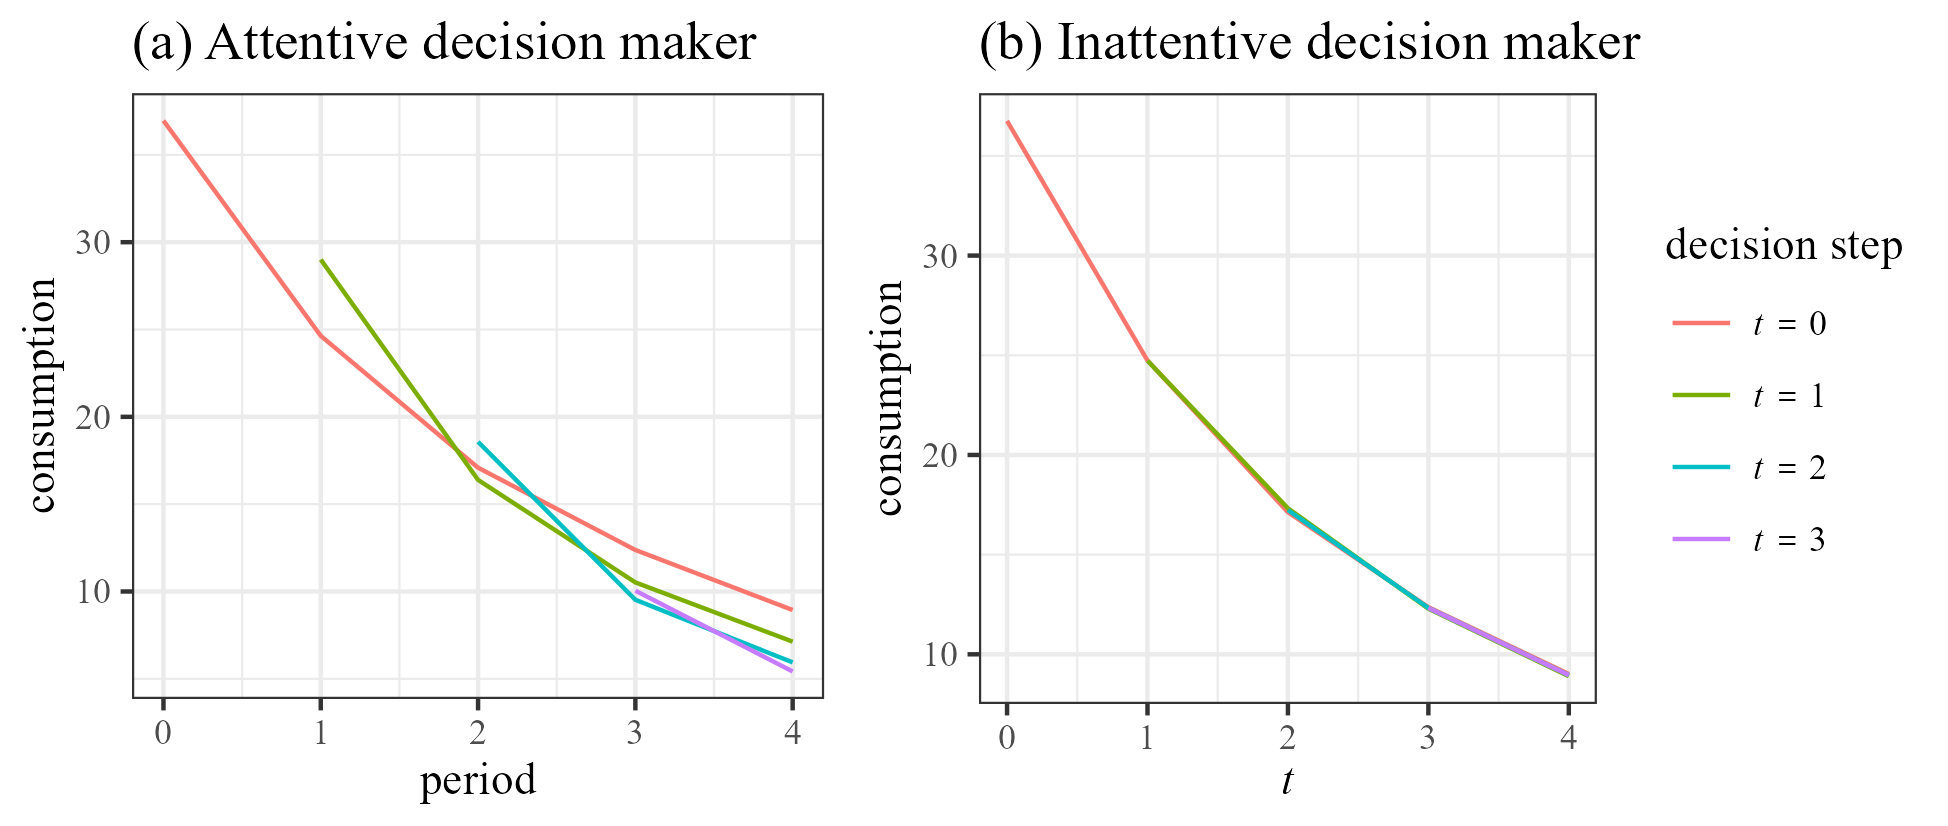
\includegraphics{images/plot-budget-dynamic.png}
  \caption{Simulation results for budget allocation. The decision maker allocations a budget of $B=100$ across five periods, $\delta=0.9$, $\lambda=70$. For each period $t$, utility funtion $u(x_t)=x_t^{0.6}$.}
  \label{fig:plot-budget-dynamic}
\end{figure}

\hypertarget{axiomization-of-adus}{%
\subsection{\texorpdfstring{Axiomization of ADUS
\label{axiom}}{Axiomization of ADUS }}\label{axiomization-of-adus}}

In this subsection, I provide an axiomatic rationale for using Shannon
cost function in ADU. I firstly define the preference relation
\(\succsim\) that can be represented by ADU, then propose four axioms to
characterize the Shannon cost function.

\textbf{Definition 2}: Preference relation \(\succsim\) has an ADU
representation if and only if, for any stochastic reward sequence
\(X_T\), \(X'_{T'}\), we have \[
X_T \succsim X'_{T'} \Longleftrightarrow U(X_T)\geq U(X'_{T'})
\]where
\(U(X_T)=\sum_{S_T\in\mathcal{S}(X_T)}\sum_{t=0}^T w(s_t)u(s_t)\),
\(U(X'_{T'})=\sum_{S_{T'}\in\mathcal{S}(X'_{T'})}\sum_{t=0}^{T'}w'(s_t)u(s_t)\).
\(S_T\) and \(S'_{T'}\) are the potential realizations of sequence
\(X_T\) and \(X'_{T'}\), \(w(.)\) and \(w'(.)\) are the solutions to the
constrained optimal discounting problems for \(X_T\) and \(X'_{T'}\).

\textbf{Axiom 1}: (\emph{state independence}) For any reward sequence
\(X_T\), \(X'_T\), \(X''_T\) and \(\alpha\in(0,1)\), \(X_T\succ X'_T\)
implies
\(\alpha X_T+ (1-\alpha)X''_T \succ \alpha X'_T + (1-\alpha) X''_T\).

Axiom 1 implies that the determination of attention weights in one
potential realization of reward sequence will not interfere that in
another. If Axiom 1 is satisfied, each state in the constrained optimal
discounting problem has an independent solution.

\textbf{Axiom 2}: \emph{(sequential outcome betweenness)} For any
non-negative real number \(b\) and deterministic reward sequence
\(S_T\), let \(S_Tb\) denote \([s_0,s_1,...,s_T,b]\), there always
exists \(\alpha\in(0,1)\) such that \(S_Tb\sim \alpha S_T+(1-\alpha)b\).

Axiom 2 implies that if we add a new element to a given sequence, the
value of the new sequence will lies between the value of the original
sequence and the utility of the newly added element. The evidence of
``violation of dominance'' \citep{scholten_better_2014} may provide
support for this axiom.

\textbf{Axiom 3}: (\emph{sequential} \emph{bracket independence}) For
any non-negative real number \(b\), \(c\) and deterministic sequence
\(S_T\), if there exist \(\alpha_1\), \(\alpha_2\), \(\alpha_3\),
\(\beta_1\), \(\beta_2\in \mathbb{R}_{>0}\) such that
\[S_Tbc\sim \alpha_1S_T+\alpha_2b+\alpha_3c \quad\text{and}\quad S_Tbc\sim \beta_1S_T+\beta_2(bc)\]
where \(bc\) denotes a sequence with immediate reward \(b\) and period-1
reward \(c\), then we must have \(\alpha_1=\beta_1\).

Axiom 3 implies that if we segment a given sequence into different
elements, and find that the value of a linear combination of these
elements is equivalent to the value of the overall sequence, then in
this linear combination, the weight for any specific element can hold
constant no matter how we segment or bracket the other elements.

\textbf{Axiom 4}: (\emph{aggregate invariance of constant sequences})
For any deterministic sequences \(S_T\), \(S'_T\), given non-negative
real number \(c'\), \(c\) and \(\alpha\in(0,1)\), if
\(\alpha s'_t+(1-\alpha)c'\succ\alpha s_t+(1-\alpha)c\) holds for every
period \(t\), then
\(\alpha S'_T+(1-\alpha)c'\succ \alpha S_T+(1-\alpha)c\).

Axiom 4 implies that in a given sequence, if the utility of every
element plus an equal amount, then the overall utility of the sequence
should plus the same amount. Note in conventional discounted utility
models, sequences are typically assumed to be separable from each other.
In that case, any sequence can be \emph{aggregate invariant}. Thus,
Axiom 4 can be viewed as a weaker version of ``separability of
sequences''.

\textbf{Theorem 1}: \(\succsim\) has an ADUS representation if and only
if it has an ADU representation and satisfies Axiom 1-4.

\hypertarget{empirical-analysis}{%
\subsection{Empirical Analysis}\label{empirical-analysis}}

\hypertarget{experimental-tests-of-attention-over-sequential-outcomes}{%
\section{Experimental Tests of Attention over Sequential
Outcomes}\label{experimental-tests-of-attention-over-sequential-outcomes}}

\hypertarget{valuation-of-risk-and-effort}{%
\section{Valuation of Risk and
Effort}\label{valuation-of-risk-and-effort}}

\hypertarget{time-schedule}{%
\section{Time Schedule}\label{time-schedule}}

\renewcommand\refname{Reference}
  \bibliography{reference.bib}

\end{document}
